\section{Competências e habilidades}\label{sec:hc}

No Brasil e no mundo, a proposta de substituir os currículos tradicionalmente baseados em conteúdo por aqueles baseados em competências e habilidades tem ganhado força.
Por exemplo, no Brasil a Base Nacional Comum Curricular (BNCC) \cite{BNCC}, homologada em 2018, ``estabelece conhecimentos, competências e habilidades que se espera que todos os estudantes desenvolvam ao longo da escolaridade básica''.

Essa abordagem tem sido adotada no ensino básico \cite{Avila2017} e superior.
De fato, ela visa a empregabilidade \cite{Butova2015}, que é também o objetivo dos cursos livres anteriormente mencionados.

Por exemplo, segundo o \foreign{EDISON Data Science Framework}, algumas competências de um cientista de dados são \cite{CF-DS-Release2019}:
\begin{compactitem}
	\item ``Usar de engenharia (geral e de software) para pesquisar, projetar, desenvolver e implementar novos instrumentos e aplicações para a coleta de dados, armazenamento, análise e visualização''.
	\item ``Utilizar eficientemente uma variedade de técnicas de análise de dados, como aprendizagem de máquina, mineração de dados, análises prescritivas e preditivas, para análise complexa de dados durante todo o ciclo de vida dos dados''
\end{compactitem}

Ademais, exemplos de habilidades são:
\begin{compactitem}
	\item ``Usar aprendizagem de máquina, tecnologia, algoritmos e ferramentas''
	\item ``Projetar experimentos, desenvolver e implementar processos de coleta de dados''
\end{compactitem}

Entretanto, as empresas frequentemente listam ferramentas e algoritmos como requisitos às vagas de trabalho que publicam, ao invés das competências e habilidades necessárias para o exercício da ciência de dados.
A Figura~\ref{fig:vagas} ilustra duas vagas dessa área, obtidas na plataforma LinkedIn.
Nela podemos ver a menção às mesmas ferramentas e algoritmos oferecidos pelos cursos livres.

\begin{figure}
	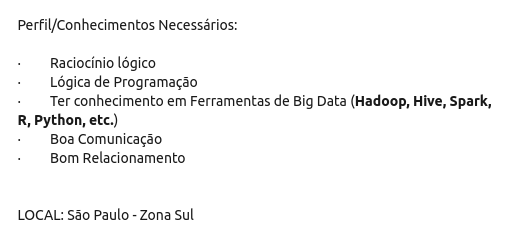
\includegraphics[width=0.45\textwidth]{eg_vaga-1_ds}\hfill
	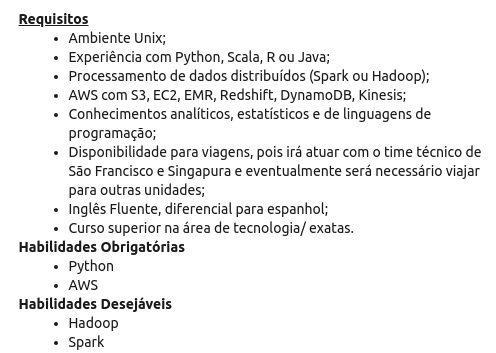
\includegraphics[width=0.45\textwidth]{eg_vaga-2_ds}
	\caption{Duas vagas de cientista de dados, extraídas do LinkedIn.}
	\label{fig:vagas}
\end{figure}